
\documentclass[11pt,spanish]{article}
\usepackage{graphicx}
\usepackage[spanish]{babel}
\usepackage[T1]{fontenc}
\usepackage[a4paper]{geometry}
\usepackage{amsmath}
\usepackage{booktabs}
\geometry{verbose,tmargin=2.5 cm,bmargin=2.5 cm,lmargin=3.5cm,rmargin=3.5cm}
\usepackage{array}
\usepackage{float}
\usepackage{graphicx}
\usepackage{subcaption}
\usepackage{url}
\captionsetup[table]{name = Tabla}
\providecommand{\abs}[1]{\lvert#1\rvert}
\providecommand{\norm}[1]{\lVert#1\rVert}

\makeatletter
\providecommand{\tabularnewline}{\\}

\def\abstractname{Resumen}
\def\refname{Referencias}
\def\figurename{\textbf{Figura}}
\def\tablename{\textbf{Tabla}}

\makeatother

\usepackage{babel}
\addto\shorthandsspanish{\spanishdeactivate{~<>}}

\begin{document}

\title{\textbf{Practical Questions: Wine Quality \& Bank Marketing}}

\author{Daniel Martínez (00329519) \\ NRC 3468}

\maketitle

% ================================================================
% PRACTICAL QUESTION 1
% ================================================================
\section{Practical Question 1 - Wine Quality}

\subsection{Análisis Exploratorio de Datos (EDA)}

Se combinaron los datasets de vino tinto (1,599 muestras) y blanco (4,898 muestras) del repositorio UCI, obteniendo 6,497 observaciones con 12 variables fisicoquímicas más un indicador de tipo de vino. No se encontraron valores nulos.

\textbf{Decisión de modelado:} Se optó por \textbf{clasificación binaria} (calidad $\geq 7$ = ``premium'', $< 7$ = ``estándar''). Justificación:
\begin{itemize}
    \item Regresión: asume intervalos iguales entre niveles de calidad (5$\to$6 equivalente a 7$\to$8), lo cual no es realista en la escala organoléptica.
    \item Multiclase: las clases extremas (3, 4, 9) contienen muy pocas muestras, generando predicciones inestables.
    \item Binaria: ofrece una decisión práctica y directa para vinicultores (``¿es este vino de calidad premium?'').
\end{itemize}

\textbf{Desbalance de clases:} El target binario presenta desbalance moderado: aproximadamente 80\% estándar y 20\% premium, lo que justifica métricas como F1 y ROC-AUC sobre accuracy simple.

\textbf{Variables clave investigadas:}
\begin{itemize}
    \item \textbf{Alcohol}: Los vinos premium presentan una mediana de alcohol claramente superior, siendo el predictor con mayor separación entre clases.
    \item \textbf{Volatile acidity}: Valores más altos de acidez volátil se asocian con menor calidad; la distribución de vinos premium está desplazada a la izquierda.
    \item \textbf{Sulphates}: Los vinos premium tienden a presentar niveles ligeramente más altos de sulfatos.
    \item \textbf{pH}: Las diferencias entre clases son menos pronunciadas, con distribuciones ampliamente superpuestas.
\end{itemize}

\begin{figure}[H]
    \centering
    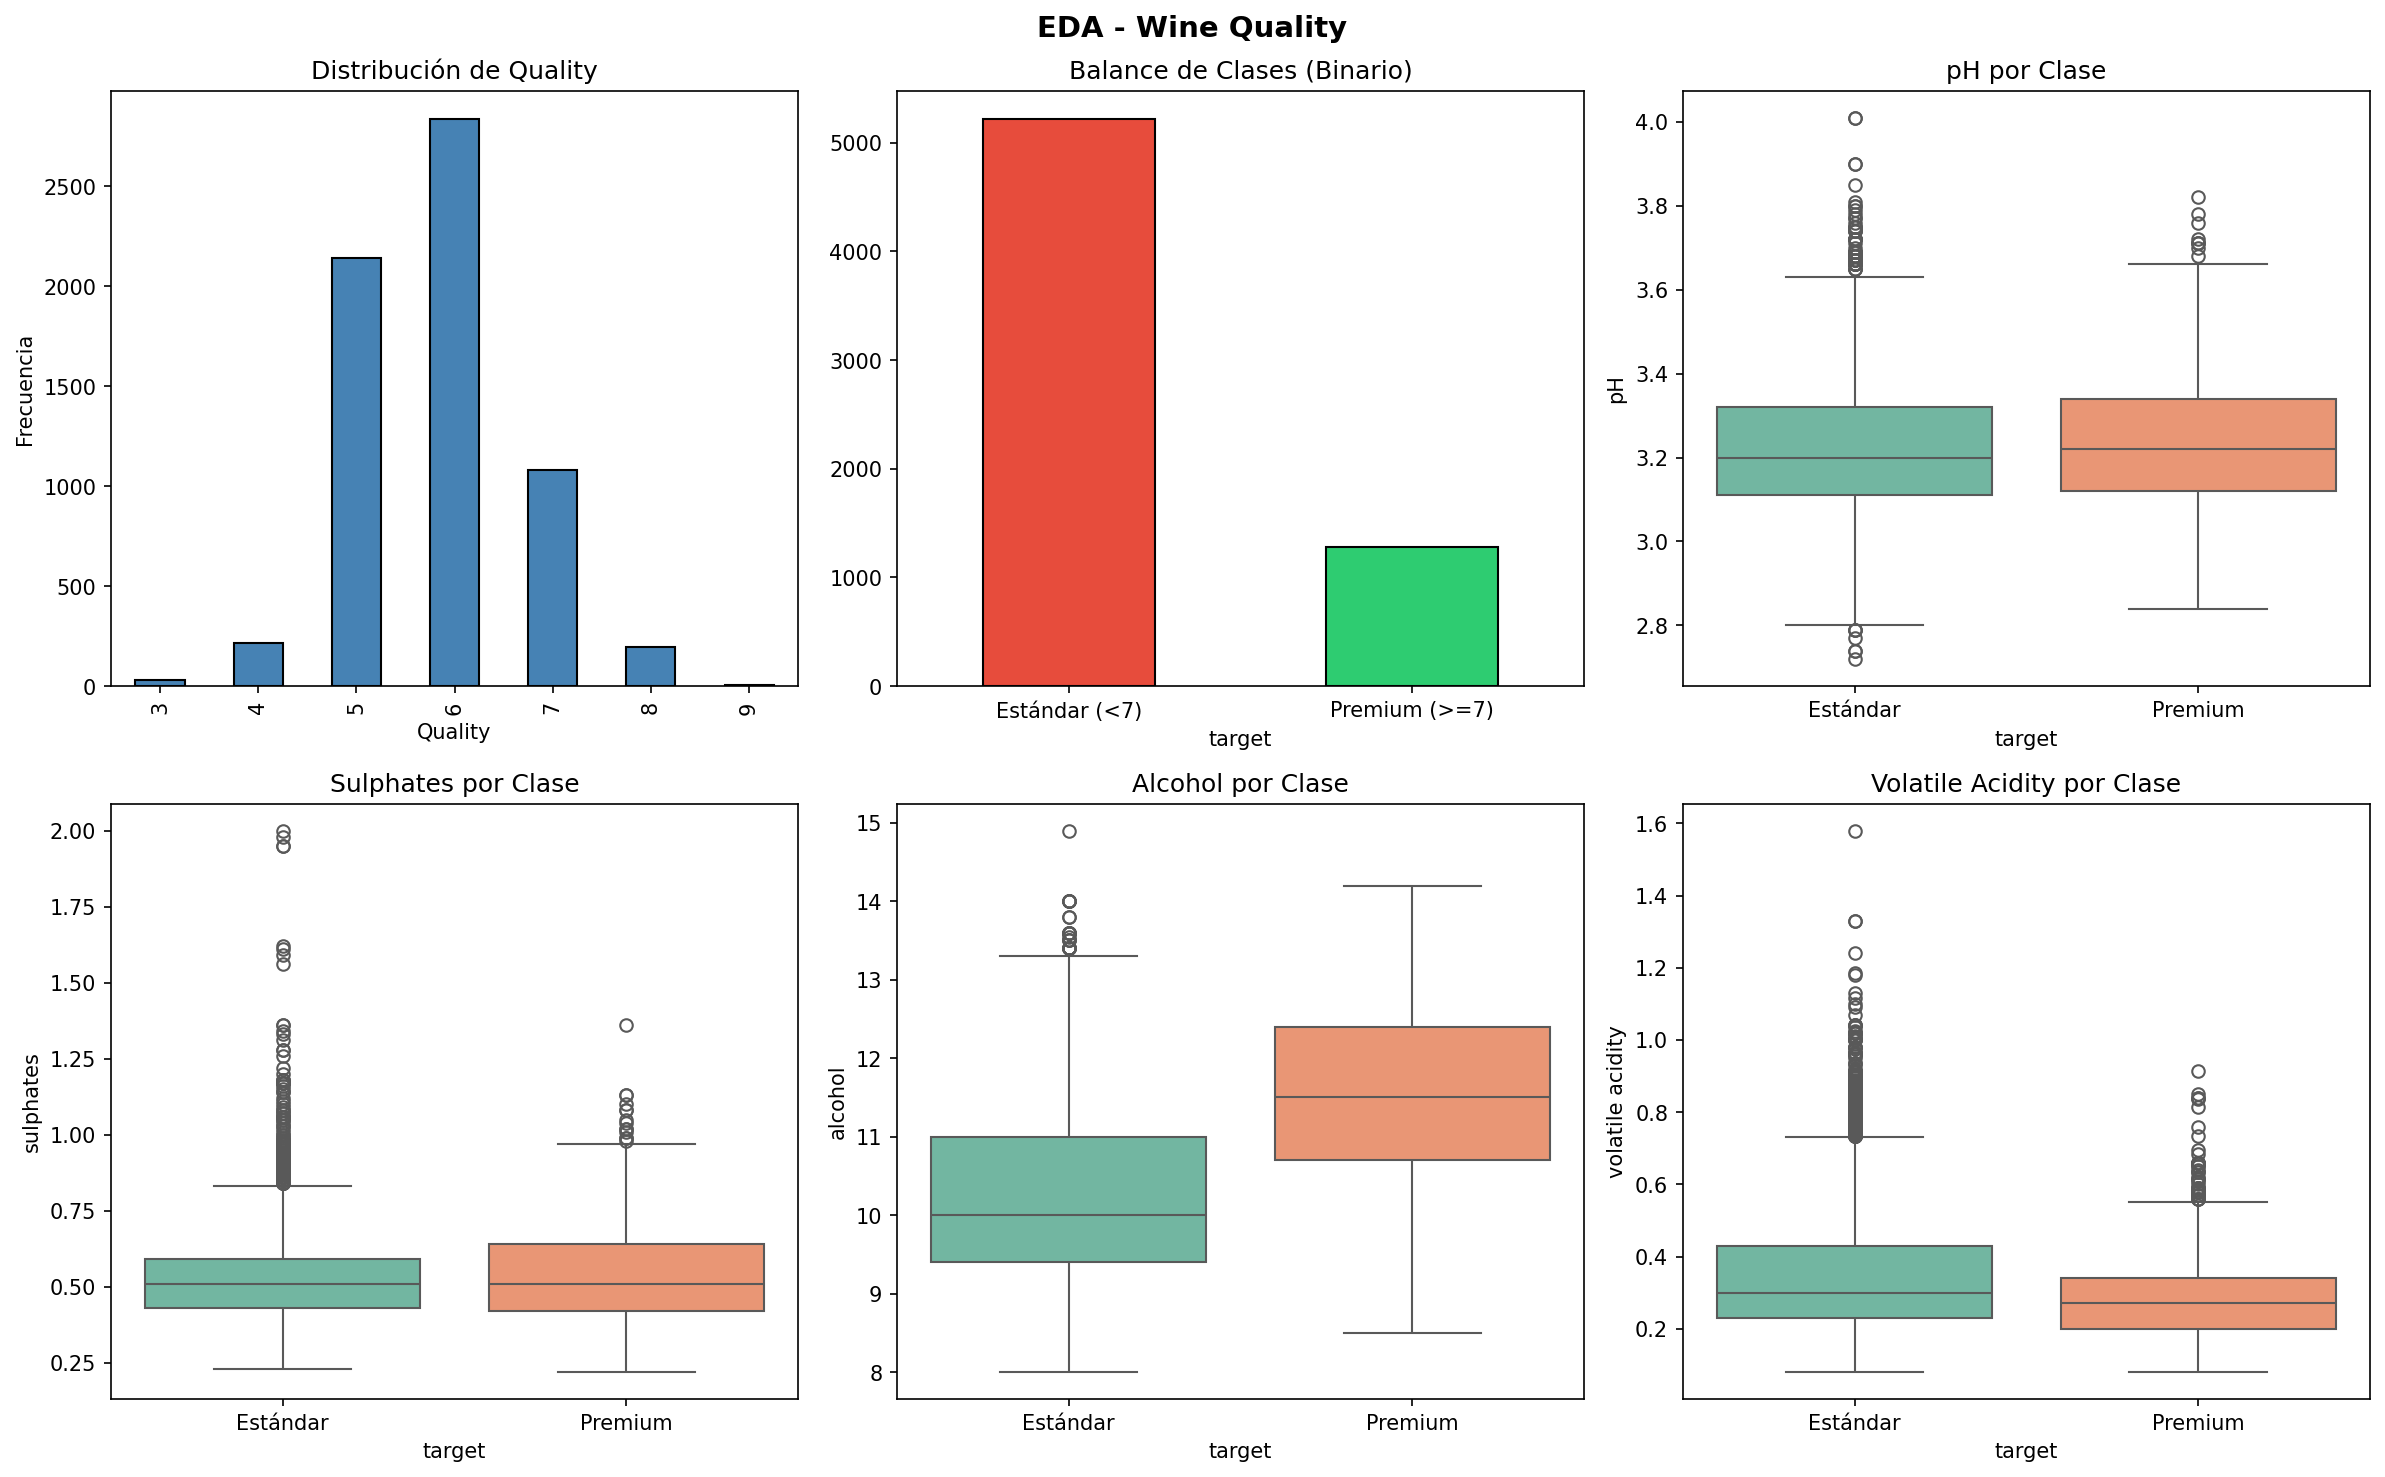
\includegraphics[scale=0.35]{eda_wine_quality.png}
    \caption{EDA: distribuciones, balance de clases y boxplots de variables clave}
    \label{fig:eda_wine}
\end{figure}

\begin{figure}[H]
    \centering
    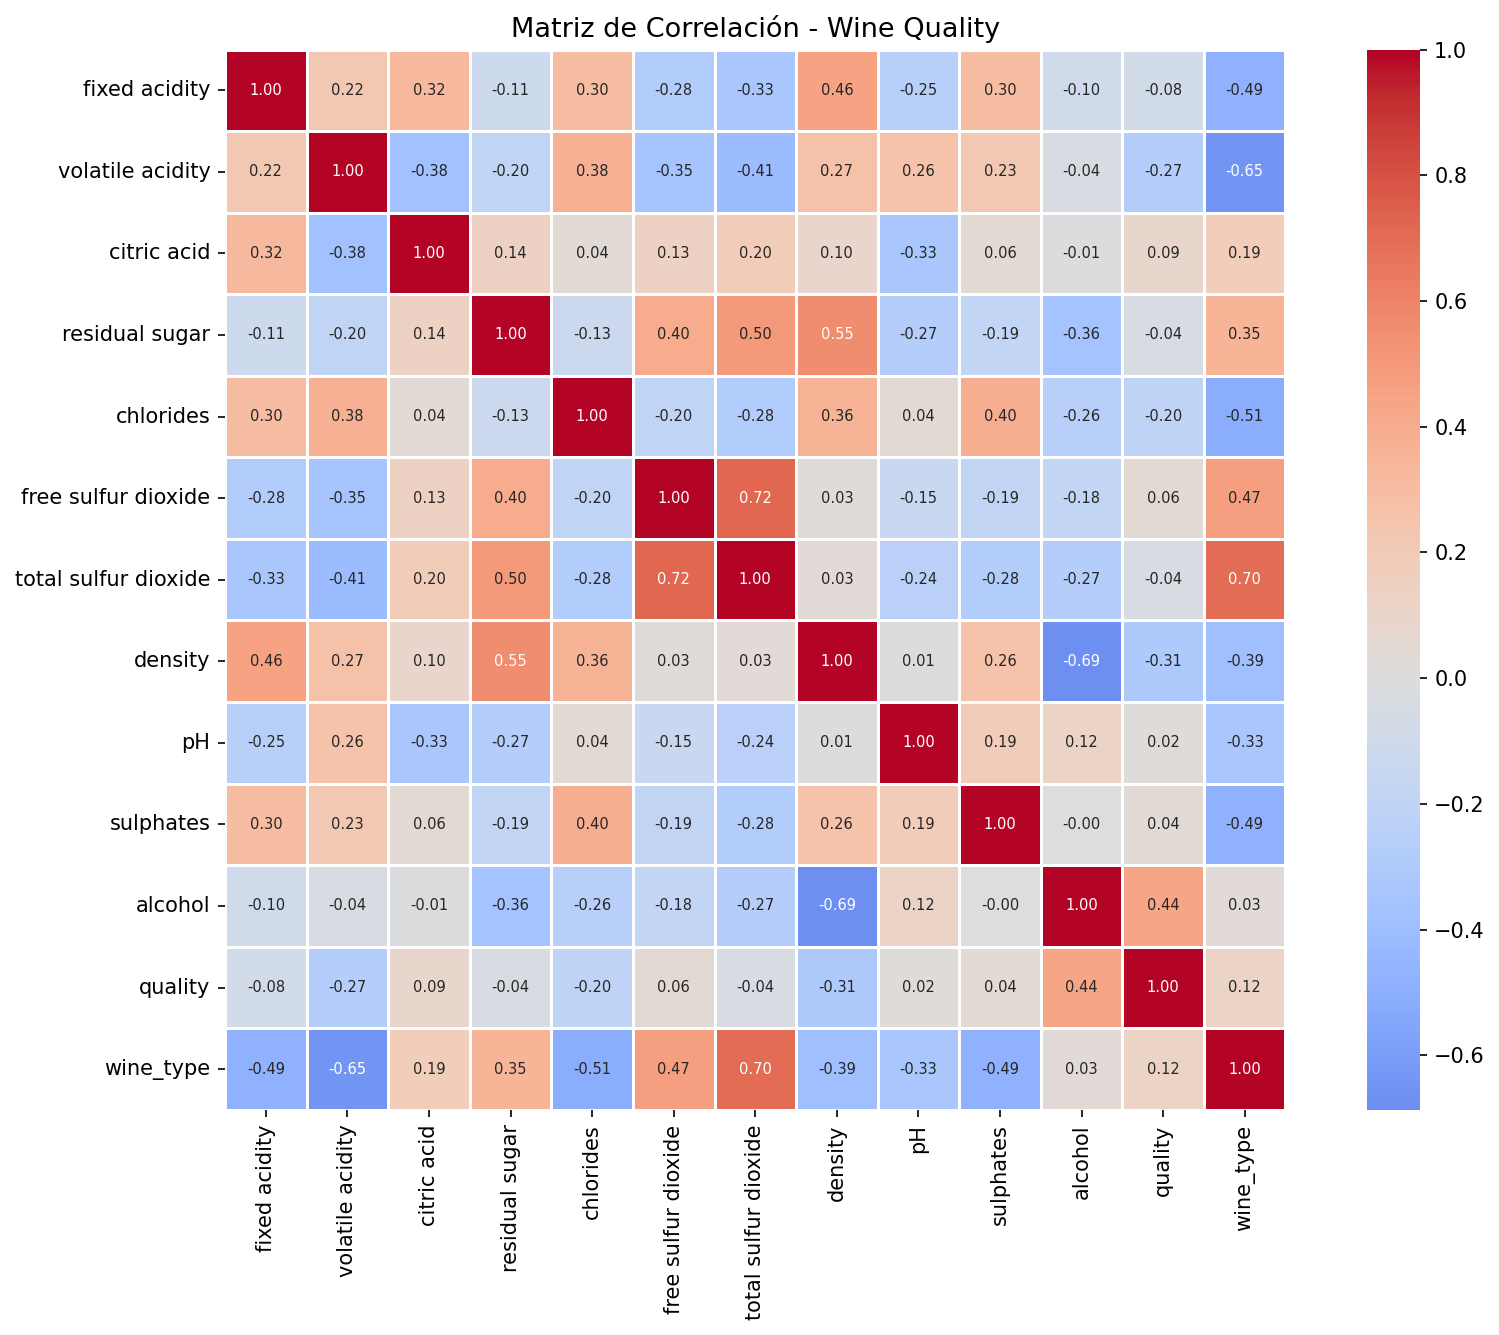
\includegraphics[scale=0.40]{corr_wine_quality.png}
    \caption{Matriz de correlación - Wine Quality}
    \label{fig:corr_wine}
\end{figure}

\subsection{Estrategia de Preprocesamiento}

\begin{itemize}
    \item \textbf{Variable wine\_type}: Codificación binaria (0=tinto, 1=blanco) como feature adicional.
    \item \textbf{Estandarización}: Se aplicó \texttt{StandardScaler} a todas las variables numéricas, requisito esencial para los modelos regularizados (Lasso, Elastic Net) y SVM, cuyas penalizaciones son sensibles a la escala.
    \item \textbf{Partición}: 80\% entrenamiento / 20\% prueba, con estratificación por clase. El set de prueba permanece aislado hasta la evaluación final.
\end{itemize}

\subsection{Diseño de Selección de Modelos}

Se empleó \textbf{Stratified 5-Fold Cross-Validation} dentro del set de entrenamiento para comparar siete modelos:

\begin{enumerate}
    \item \textbf{Ridge (L2)}: Regresión logística con penalización $\lambda\norm{\beta}^2_2$. Reduce sobreajuste sin seleccionar variables.
    \item \textbf{Lasso (L1)}: Regresión logística con penalización $\lambda\norm{\beta}_1$. Realiza selección automática de variables (coeficientes = 0).
    \item \textbf{Elastic Net}: Combinación $\alpha\norm{\beta}_1 + (1-\alpha)\norm{\beta}^2_2$. Estabiliza la selección cuando hay variables correlacionadas.
    \item \textbf{Decision Tree}: Modelo basado en particiones recursivas. Interpretable pero propenso a alta varianza.
    \item \textbf{Random Forest}: Ensamble de árboles con bagging. Reduce varianza y mejora generalización.
    \item \textbf{SVM (RBF)}: Máquina de vectores de soporte con kernel gaussiano. Efectivo en espacios de alta dimensión.
    \item \textbf{Red Neuronal}: Perceptrón multicapa (MLP) con arquitectura (32, 16) neuronas y early stopping.
\end{enumerate}

La métrica principal de selección fue el \textbf{F1-Score}, dado el desbalance de clases. Se realizó \texttt{GridSearchCV} para afinar hiperparámetros de Random Forest ($n\_estimators$, $max\_depth$), SVM ($C$, $\gamma$) y Ridge ($C$).

\subsection{Comparación de Modelos Tuneados}

\begin{figure}[H]
    \centering
    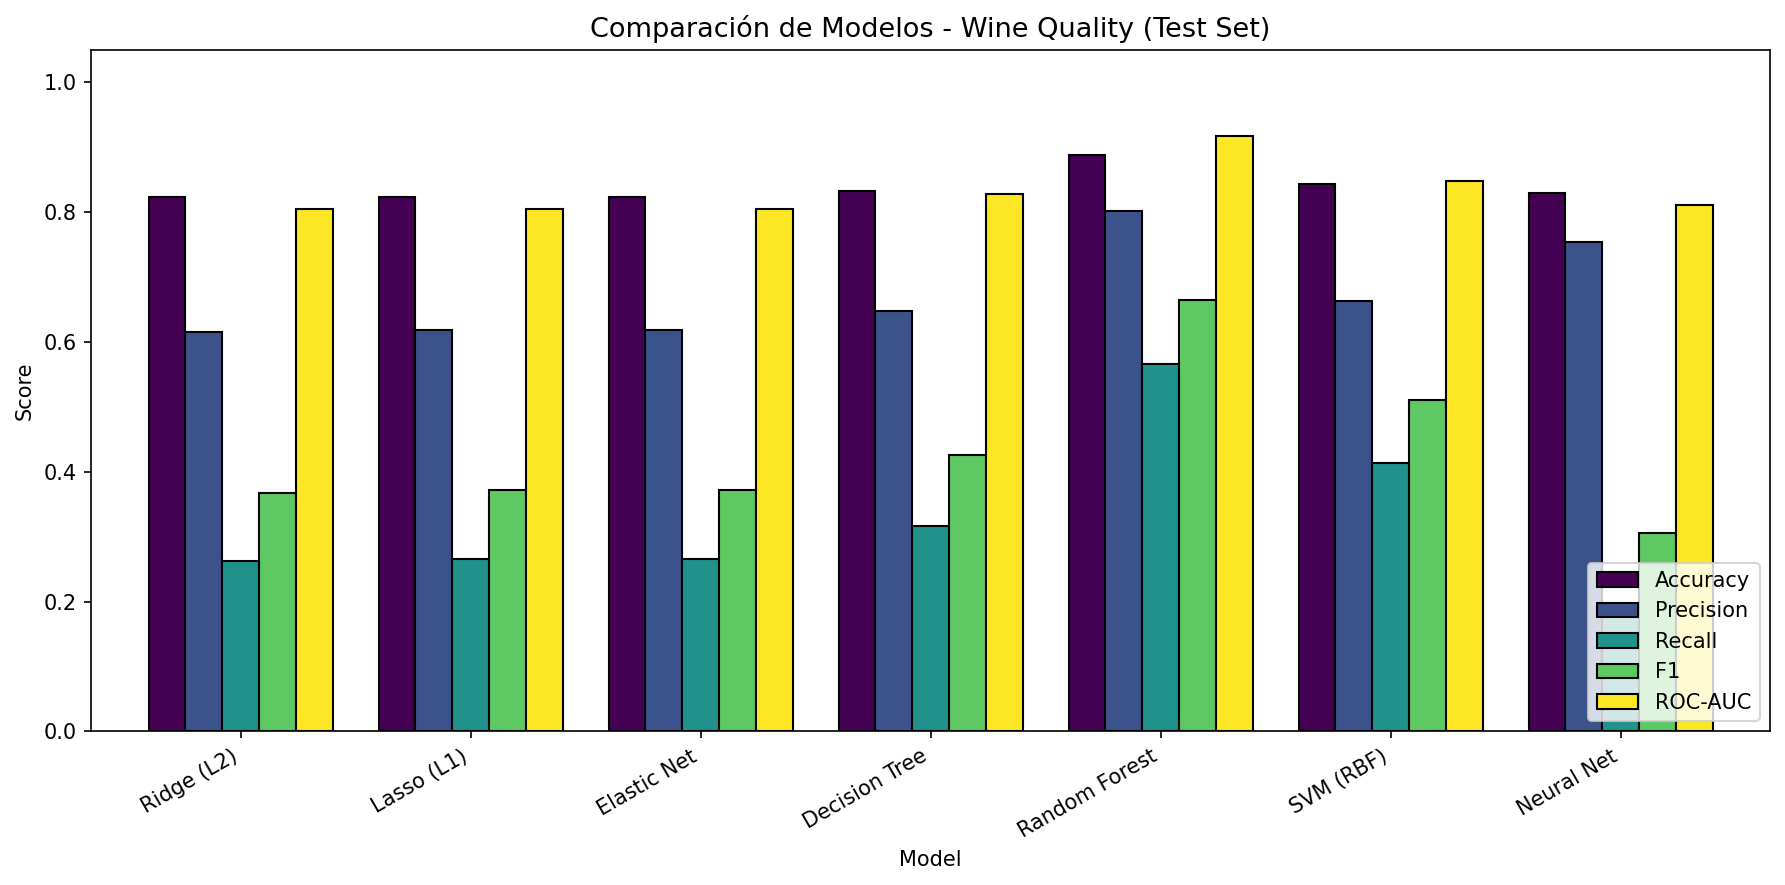
\includegraphics[scale=0.40]{comparacion_modelos_wine.png}
    \caption{Comparación de métricas en test set - Wine Quality}
    \label{fig:comp_wine}
\end{figure}

\begin{figure}[H]
    \centering
    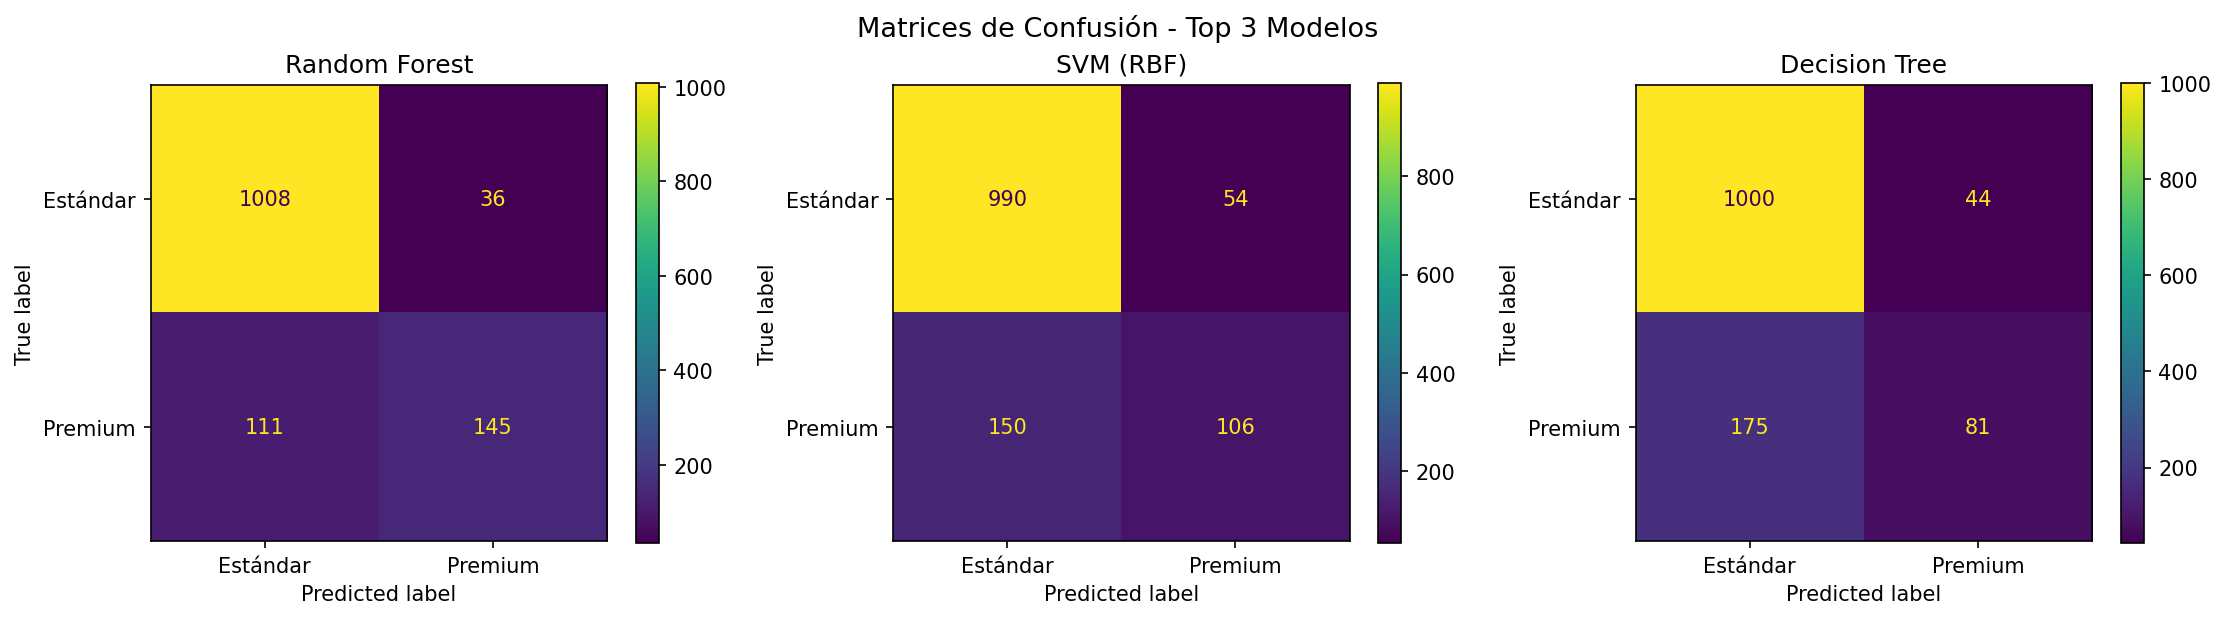
\includegraphics[scale=0.40]{confusion_matrices_wine.png}
    \caption{Matrices de confusión de los 3 mejores modelos}
    \label{fig:cm_wine}
\end{figure}

\subsection{Estabilidad de Predictores: Lasso vs Elastic Net}

Se entrenaron modelos Lasso y Elastic Net para múltiples valores de regularización $C \in \{0.01, 0.05, 0.1, 0.5, 1, 5, 10\}$ y se trazaron las trayectorias de coeficientes.

\textbf{Hallazgo principal}: Elastic Net exhibe trayectorias más suaves y estables. Cuando variables están correlacionadas (e.g., \textit{free sulfur dioxide} y \textit{total sulfur dioxide}), Lasso selecciona arbitrariamente una y descarta la otra, mientras que Elastic Net distribuye el peso entre ambas gracias a la componente L2. Esto se evidencia en una menor varianza de los coeficientes a lo largo de los valores de $C$.

\begin{figure}[H]
    \centering
    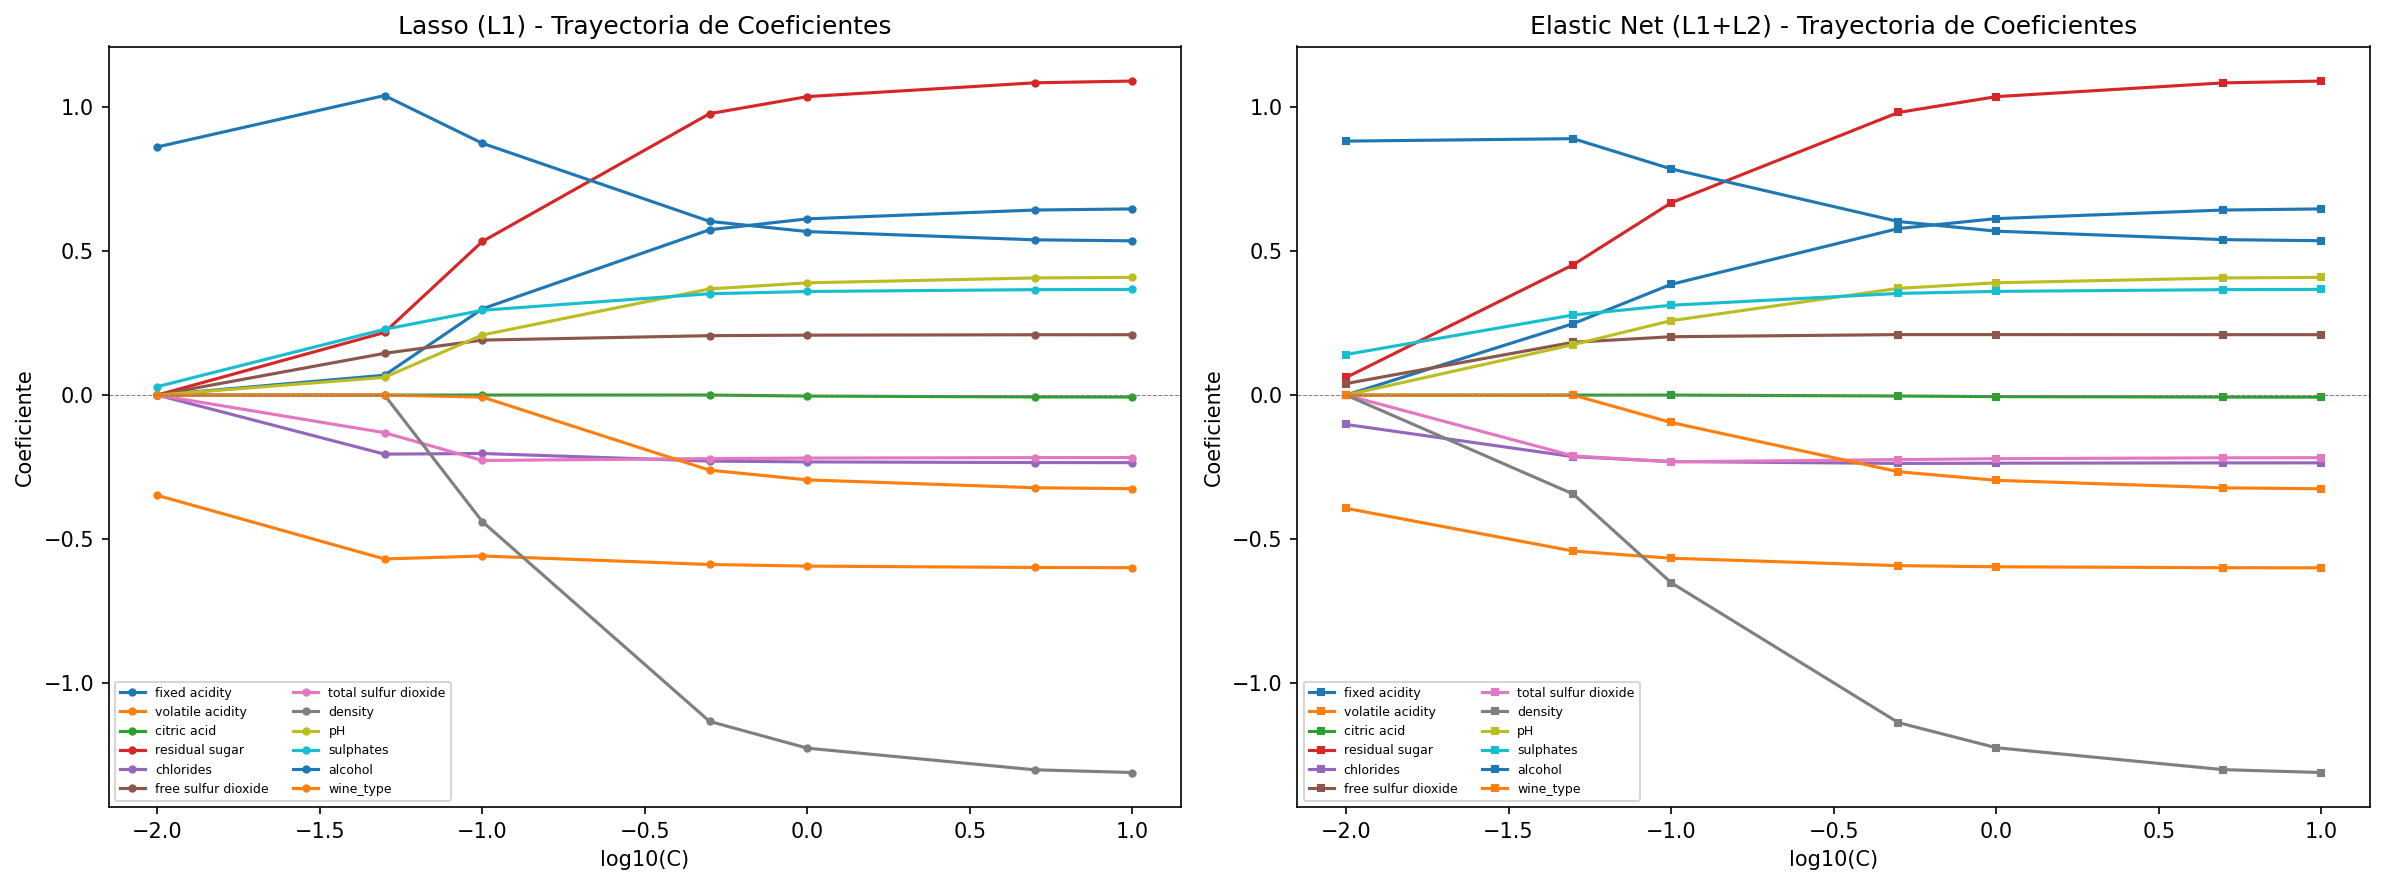
\includegraphics[scale=0.38]{lasso_vs_elasticnet_wine.png}
    \caption{Trayectoria de coeficientes: Lasso (L1) vs Elastic Net}
    \label{fig:lasso_enet}
\end{figure}

\subsection{Evaluación Final en Test Set}

El modelo final se evalúa en el set de prueba aislado. Las métricas reportadas son: Accuracy, Precision, Recall, F1-Score y ROC-AUC.

\textbf{Modelo recomendado}: El Random Forest tuneado presenta el mejor balance entre precisión y recall (mayor F1 y ROC-AUC), seguido por la red neuronal y SVM.

\subsection{Interpretación e Inferencia}

\begin{figure}[H]
    \centering
    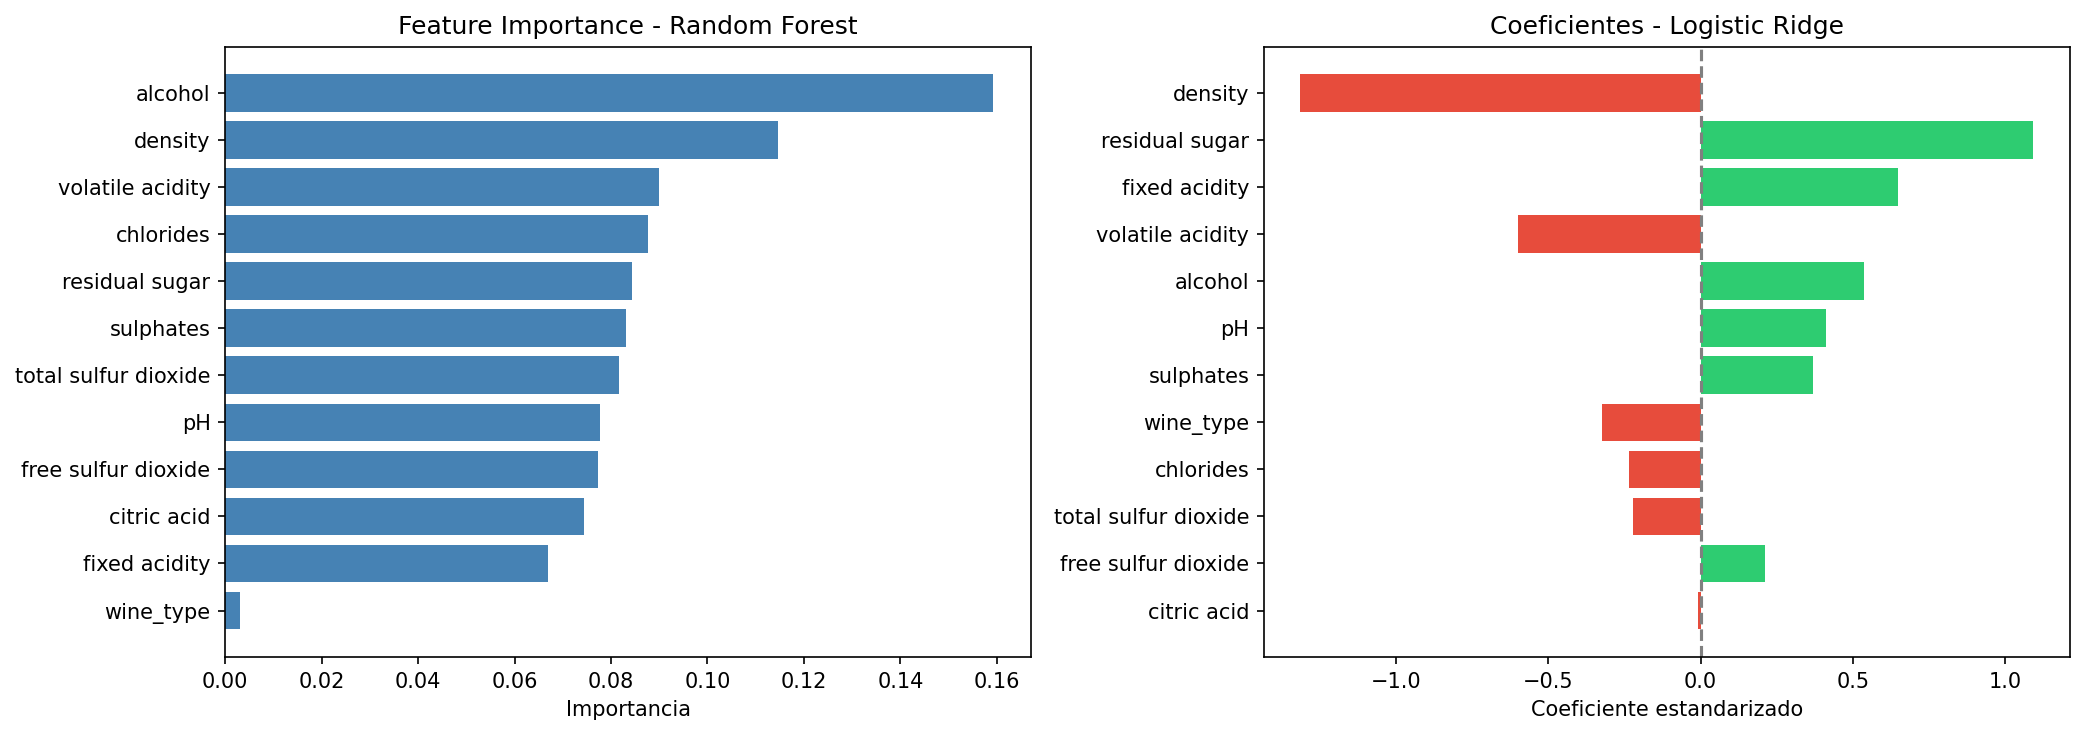
\includegraphics[scale=0.38]{feature_importance_wine.png}
    \caption{Feature importance (RF) y coeficientes estandarizados (Ridge)}
    \label{fig:fi_wine}
\end{figure}

\textbf{Interpretación para vinicultores (asociacional, no causal):}
\begin{itemize}
    \item El \textbf{alcohol} es el predictor más fuerte: vinos con mayor contenido alcohólico están asociados con calificaciones premium.
    \item La \textbf{acidez volátil} tiene efecto negativo: niveles altos se asocian con menor calidad percibida.
    \item Los \textbf{sulfatos} contribuyen positivamente a la clasificación como premium.
    \item El \textbf{tipo de vino} (tinto vs blanco) influye en la predicción, reflejando diferencias sistemáticas entre ambas categorías.
\end{itemize}

\subsection{Ejemplos de Predicción}

Se presentan 5 predicciones del set de prueba con el modelo seleccionado (Random Forest tuneado), mostrando la clase real, la predicción y la probabilidad estimada $P(\text{Premium})$. Se realizó un muestreo estratificado para incluir ejemplos de ambas clases.

\begin{table}[H]
\centering
\caption{Ejemplos de predicción - Wine Quality (Random Forest)}
\label{tab:pred_wine}
\begin{tabular}{ccccc}
\toprule
\textbf{\#} & \textbf{Real} & \textbf{Predicción} & \textbf{$P(\text{Premium})$} & \textbf{Correcto} \\
\midrule
1 & Premium  & Premium  & 0.7300 & Sí \\
2 & Estándar & Estándar & 0.1400 & Sí \\
3 & Estándar & Estándar & 0.0150 & Sí \\
4 & Estándar & Estándar & 0.0850 & Sí \\
5 & Premium  & Premium  & 0.6400 & Sí \\
\bottomrule
\end{tabular}
\end{table}

El modelo clasifica correctamente los 5 ejemplos mostrados, con probabilidades claramente diferenciadas: los vinos premium obtienen $P > 0.6$ mientras que los estándar se mantienen por debajo de $0.15$, lo que demuestra una buena separación de clases en el score predictivo.

% ================================================================
% PRACTICAL QUESTION 2
% ================================================================
\section{Practical Question 2 - Bank Marketing}

\subsection{Análisis Exploratorio de Datos (EDA)}

El dataset Bank Marketing del UCI contiene 41,188 registros de campañas de telemarketing de un banco portugués. El objetivo es predecir si un cliente suscribirá un depósito a plazo (\textit{y}: yes/no).

\textbf{Desbalance de clases:} Severo desbalance con $\sim$88.7\% ``no'' y $\sim$11.3\% ``sí''. Esto exige métricas como ROC-AUC y PR-AUC en lugar de accuracy.

\textbf{Variables categóricas y valores missing-like:}
\begin{itemize}
    \item Variables como \textit{job}, \textit{marital}, \textit{education}, \textit{default}, \textit{housing}, \textit{loan} contienen niveles ``unknown'' que actúan como valores faltantes.
    \item \textit{default} presenta la mayor proporción de ``unknown'' ($\sim$20\%).
    \item Se tratan los ``unknown'' como NaN y se imputan con la moda.
\end{itemize}

\textbf{Variables de campaña/contacto:}
\begin{itemize}
    \item \textit{campaign}: Número de contactos en la campaña actual (mediana $\sim$2-3).
    \item \textit{pdays}: Días desde el último contacto (999 = nunca contactado antes).
    \item \textit{previous}: Número de contactos en campañas previas.
    \item \textit{poutcome}: Resultado de la campaña anterior; \textit{success} presenta la mayor tasa de conversión.
\end{itemize}

\begin{figure}[H]
    \centering
    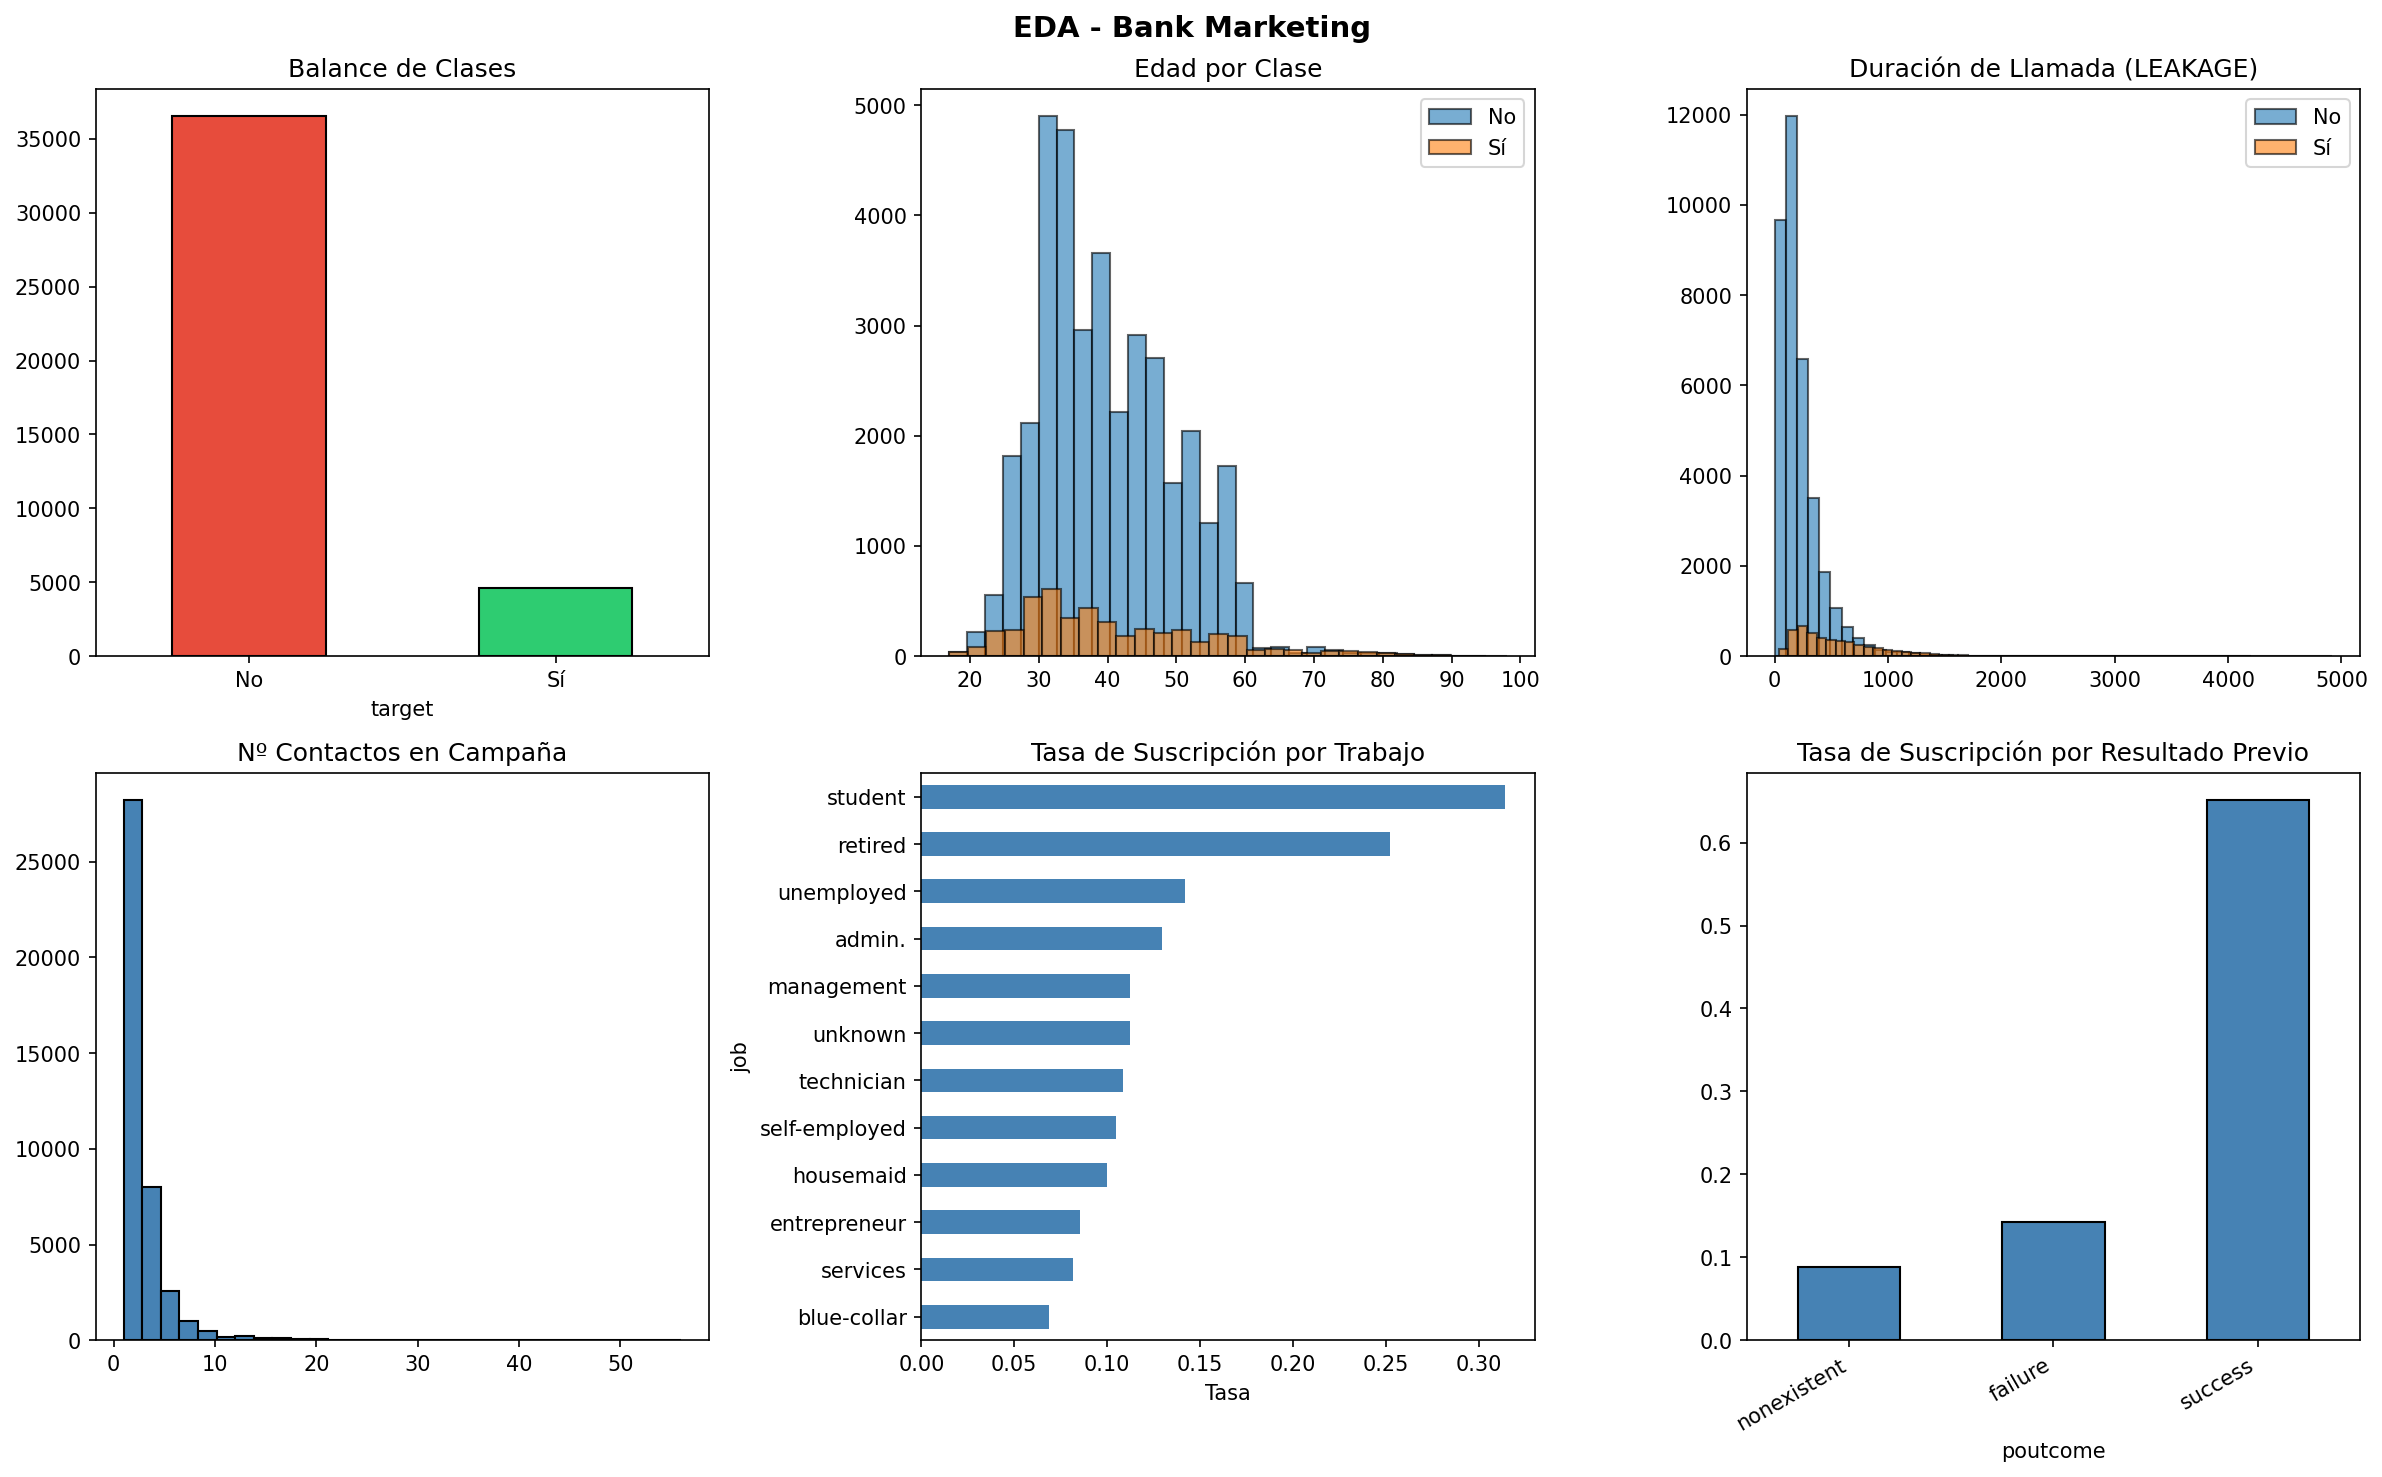
\includegraphics[scale=0.35]{eda_bank_marketing.png}
    \caption{EDA: balance de clases, distribuciones y tasas de suscripción}
    \label{fig:eda_bank}
\end{figure}

\begin{figure}[H]
    \centering
    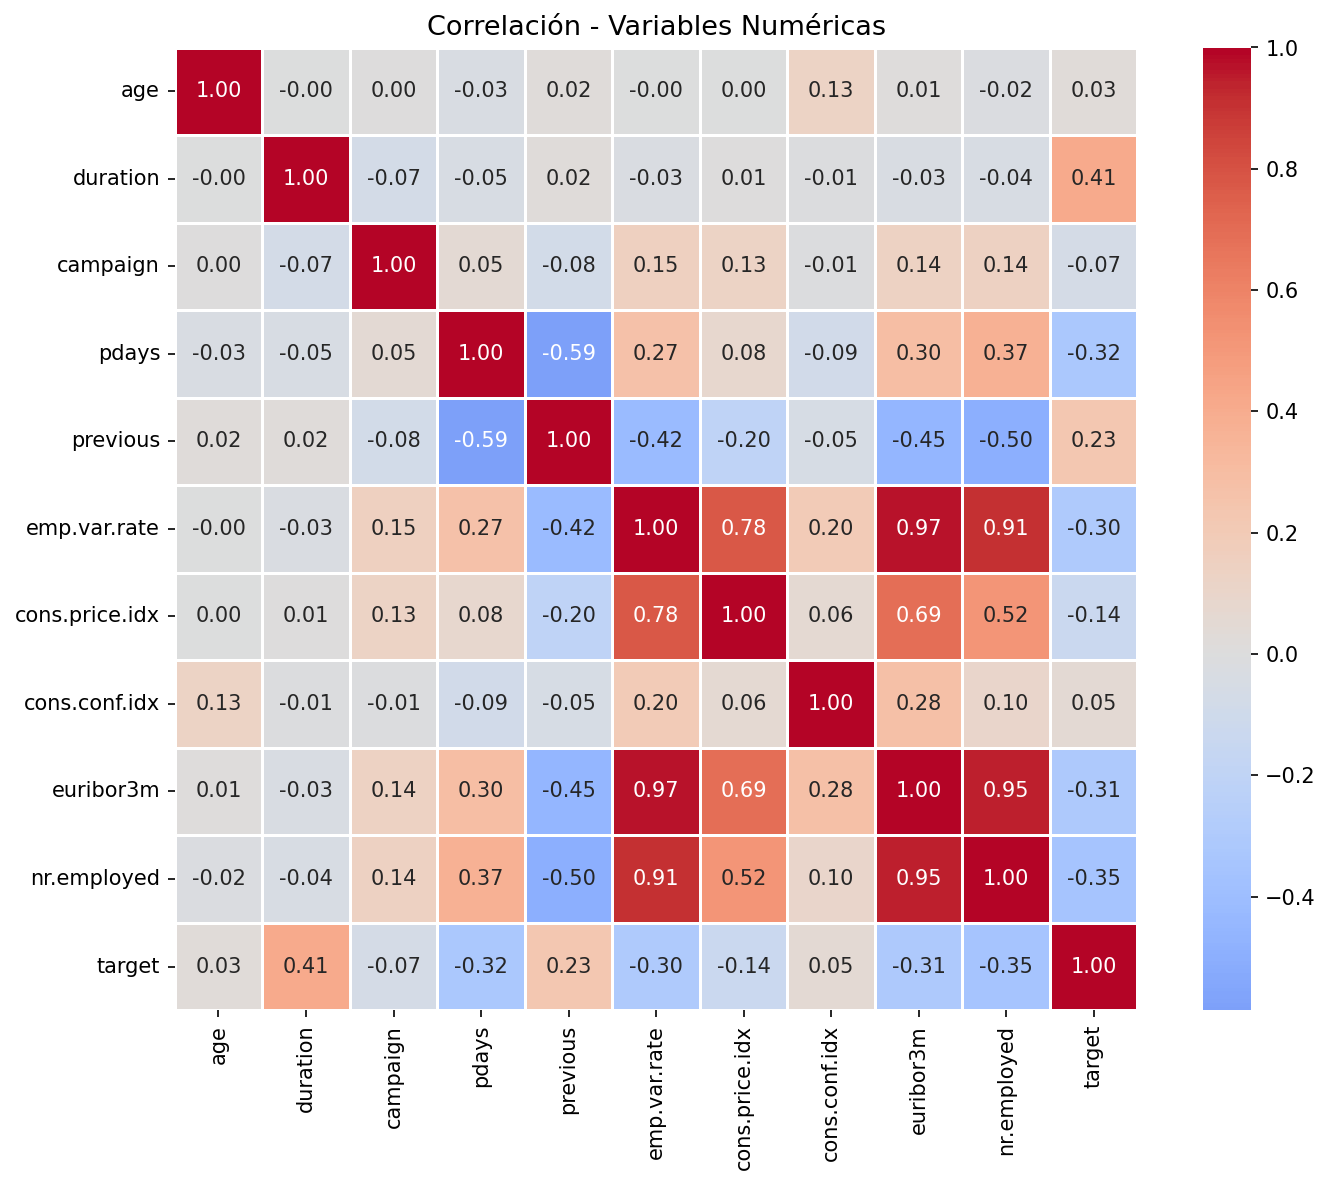
\includegraphics[scale=0.42]{corr_bank_marketing.png}
    \caption{Correlación de variables numéricas - Bank Marketing}
    \label{fig:corr_bank}
\end{figure}

\subsection{Pipeline de Preprocesamiento}

\textbf{Chequeo de leakage -- variable \textit{duration}:}

La variable \textit{duration} (duración de la última llamada) es un caso clásico de \textbf{data leakage}. Solo se conoce \textit{después} de realizar la llamada, por lo que no puede usarse para predecir \textit{antes} de contactar al cliente. Incluirla infla artificialmente las métricas. Se removió del pipeline.

\textbf{Pipeline implementado:}
\begin{itemize}
    \item \textbf{Variables numéricas}: Imputación por mediana + estandarización con \texttt{StandardScaler}.
    \item \textbf{Variables categóricas}: Imputación por moda + \texttt{OneHotEncoder} (drop=`first' para evitar multicolinealidad).
    \item \textbf{Orquestación}: \texttt{ColumnTransformer} + \texttt{Pipeline} de scikit-learn para prevenir leakage entre train y test.
    \item \textbf{Partición}: 80\%/20\% con estratificación por clase.
\end{itemize}

\subsection{Diseño de Selección de Modelos}

Se compararon siete modelos con \textbf{Stratified 5-Fold CV}:
\begin{enumerate}
    \item Ridge (L2), Lasso (L1), Elastic Net: Modelos lineales regularizados.
    \item Decision Tree ($max\_depth=5$).
    \item Random Forest (tuneado vía GridSearchCV).
    \item SVM con kernel lineal (eficiente para datasets grandes).
    \item Red Neuronal MLP (64, 32) con early stopping.
\end{enumerate}

Se evaluaron simultáneamente: ROC-AUC, F1, Recall y Precision en cada fold.

\subsection{Comparación de Modelos Tuneados}

\begin{figure}[H]
    \centering
    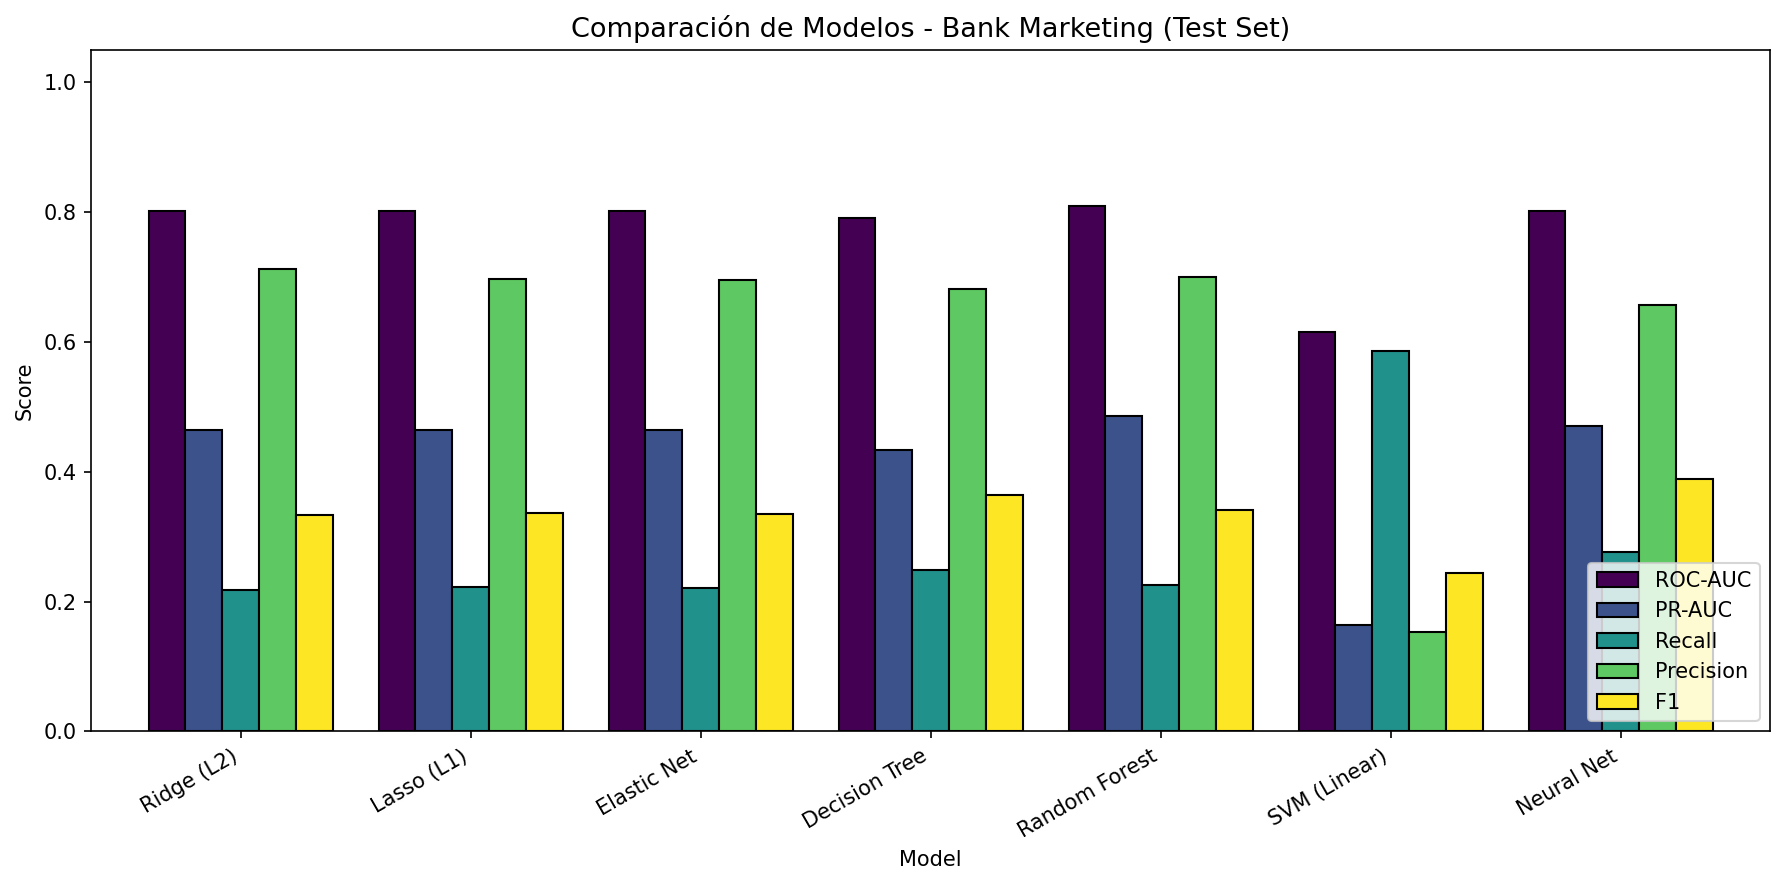
\includegraphics[scale=0.38]{comparacion_modelos_bank.png}
    \caption{Comparación de métricas en test set - Bank Marketing}
    \label{fig:comp_bank}
\end{figure}

\begin{figure}[H]
    \centering
    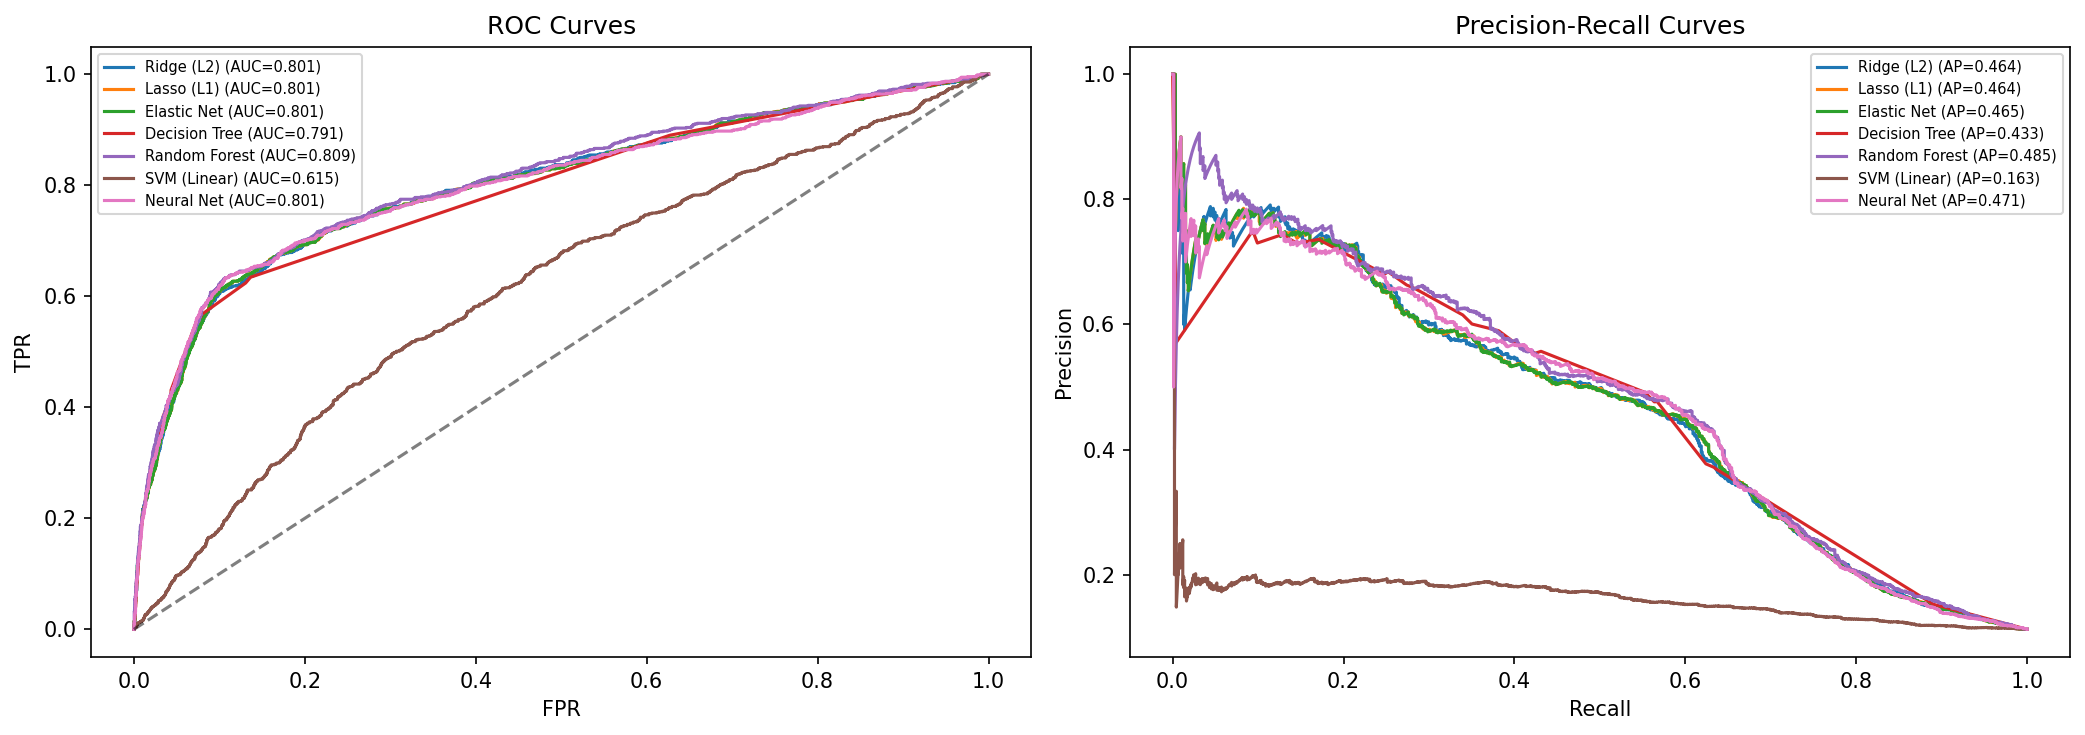
\includegraphics[scale=0.38]{roc_pr_curves_bank.png}
    \caption{Curvas ROC y Precision-Recall}
    \label{fig:roc_pr}
\end{figure}

\subsection{Evaluación Final en Test Set}

Se reportan ROC-AUC, PR-AUC, Recall, Precision, F1 y matrices de confusión a múltiples umbrales de decisión (0.3, 0.5, 0.7) para evaluar el trade-off operativo.

\begin{figure}[H]
    \centering
    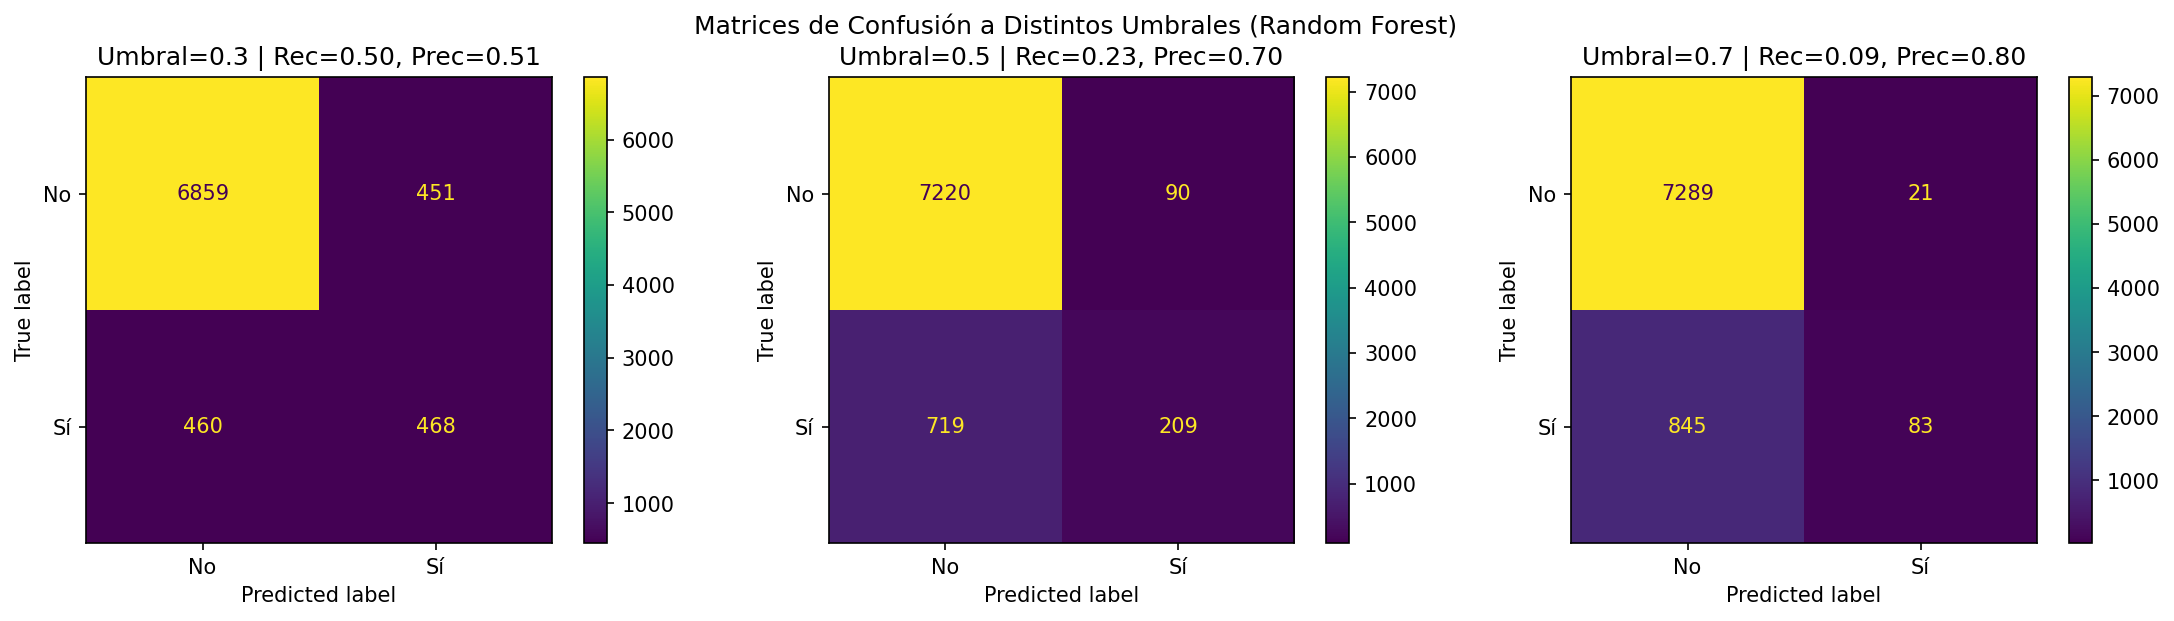
\includegraphics[scale=0.38]{confusion_thresholds_bank.png}
    \caption{Matrices de confusión a distintos umbrales de negocio}
    \label{fig:cm_bank}
\end{figure}

Un umbral más bajo (0.3) captura más suscriptores potenciales (mayor recall) a costa de más falsos positivos, mientras que un umbral alto (0.7) es conservador pero pierde oportunidades.

\subsection{Interpretación e Inferencia}

\begin{figure}[H]
    \centering
    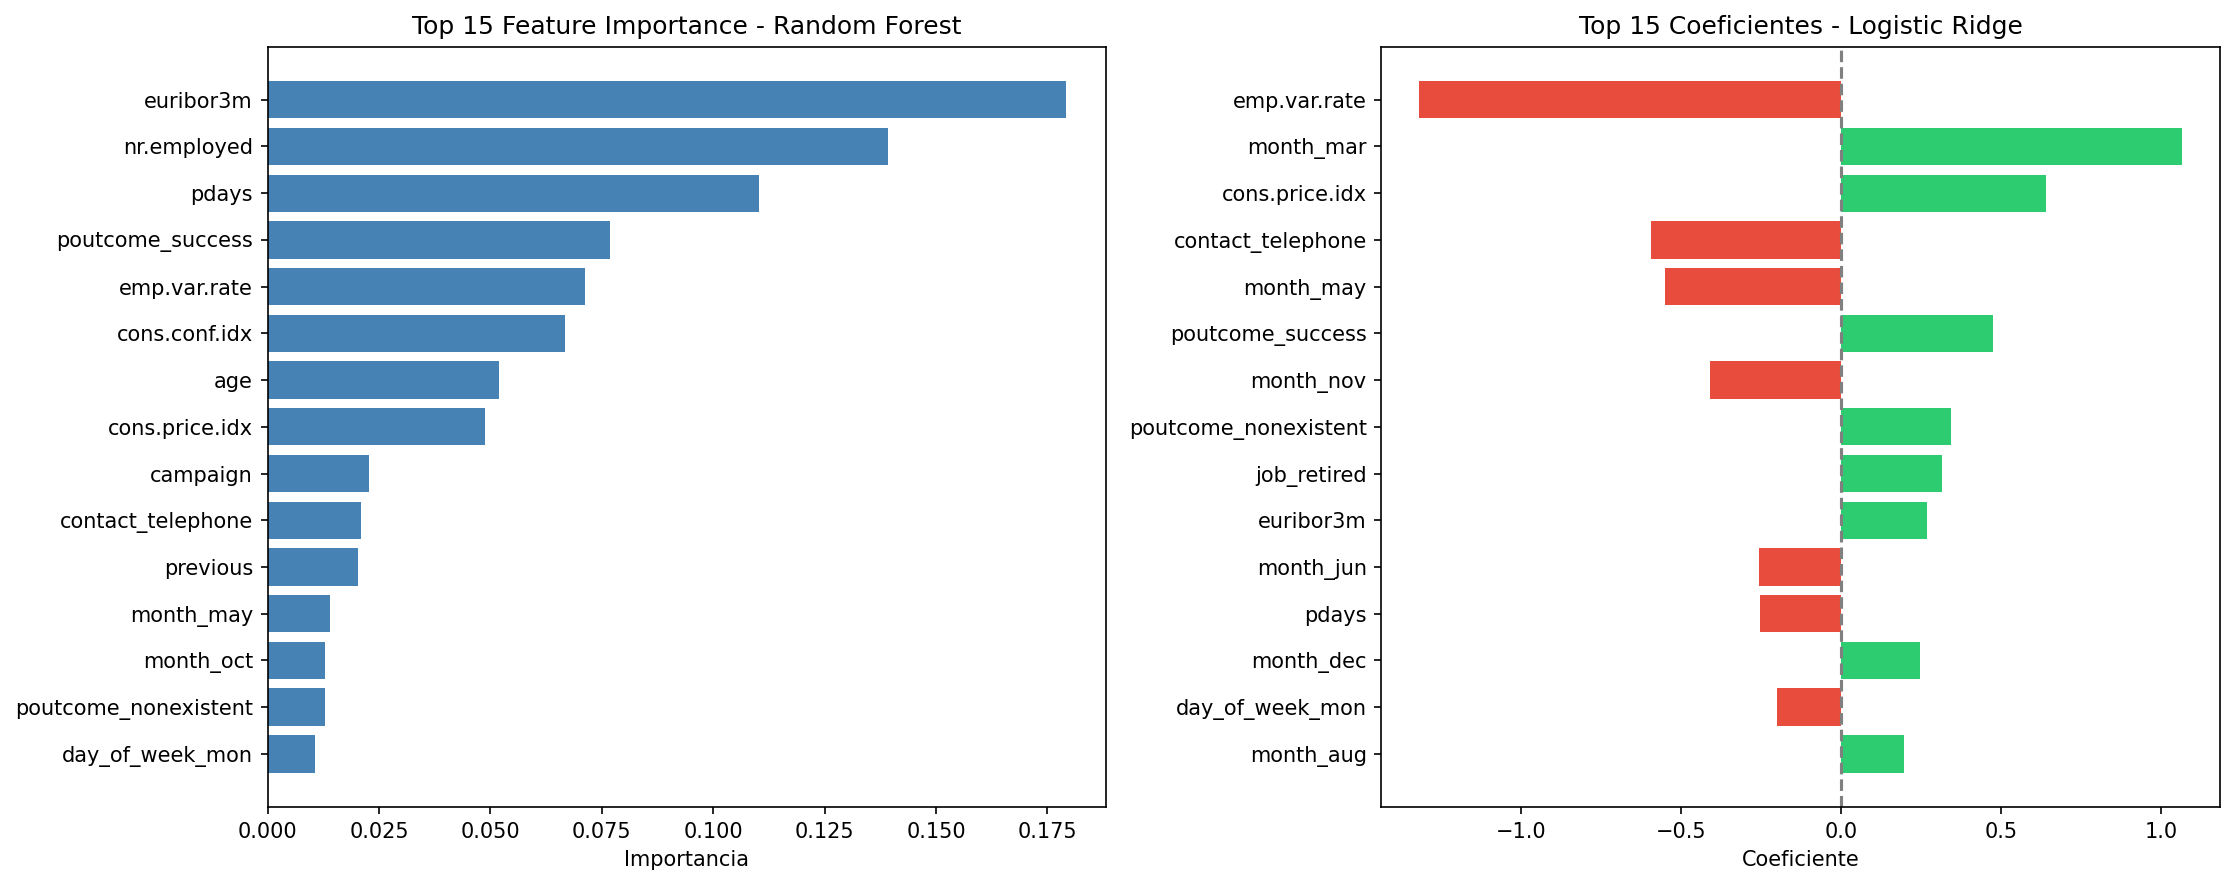
\includegraphics[scale=0.38]{feature_importance_bank.png}
    \caption{Top 15 features: RF importance y coeficientes logísticos}
    \label{fig:fi_bank}
\end{figure}

\textbf{Interpretación (asociacional, sin claims causales de marketing):}
\begin{itemize}
    \item Variables \textbf{macroeconómicas} (\textit{euribor3m}, \textit{nr.employed}, \textit{emp.var.rate}) dominan: reflejan el contexto económico del momento de la campaña, no el efecto directo del marketing.
    \item \textit{poutcome\_success}: Clientes con historial exitoso de conversión previa presentan la mayor asociación positiva.
    \item \textit{contact\_telephone}: El canal celular muestra mejores tasas que el teléfono fijo.
    \item No se puede afirmar que ``llamar más veces causa suscripción''; la correlación puede reflejar sesgo de selección (se insiste más con clientes que muestran interés).
\end{itemize}

\subsection{Recomendación de Estrategia de Contacto}

Bajo capacidad limitada de call center:

\begin{enumerate}
    \item \textbf{Priorización por score}: Ordenar clientes por $P(\text{suscripción})$ descendente y contactar solo al top-K según capacidad disponible.
    \item \textbf{Umbral operativo}: Un umbral de 0.30 maximiza recall sin desperdiciar excesivos recursos en falsos positivos.
    \item \textbf{Segmentación}:
    \begin{itemize}
        \item Alta prioridad: Clientes con \textit{poutcome}=success.
        \item Media prioridad: Clientes jóvenes/jubilados con alto score.
        \item Baja prioridad: Clientes con múltiples contactos previos sin éxito.
    \end{itemize}
    \item \textbf{Curva de captura (Lift)}: Contactando al top 20\% por score se espera capturar más del 50\% de las suscripciones potenciales.
\end{enumerate}

\begin{figure}[H]
    \centering
    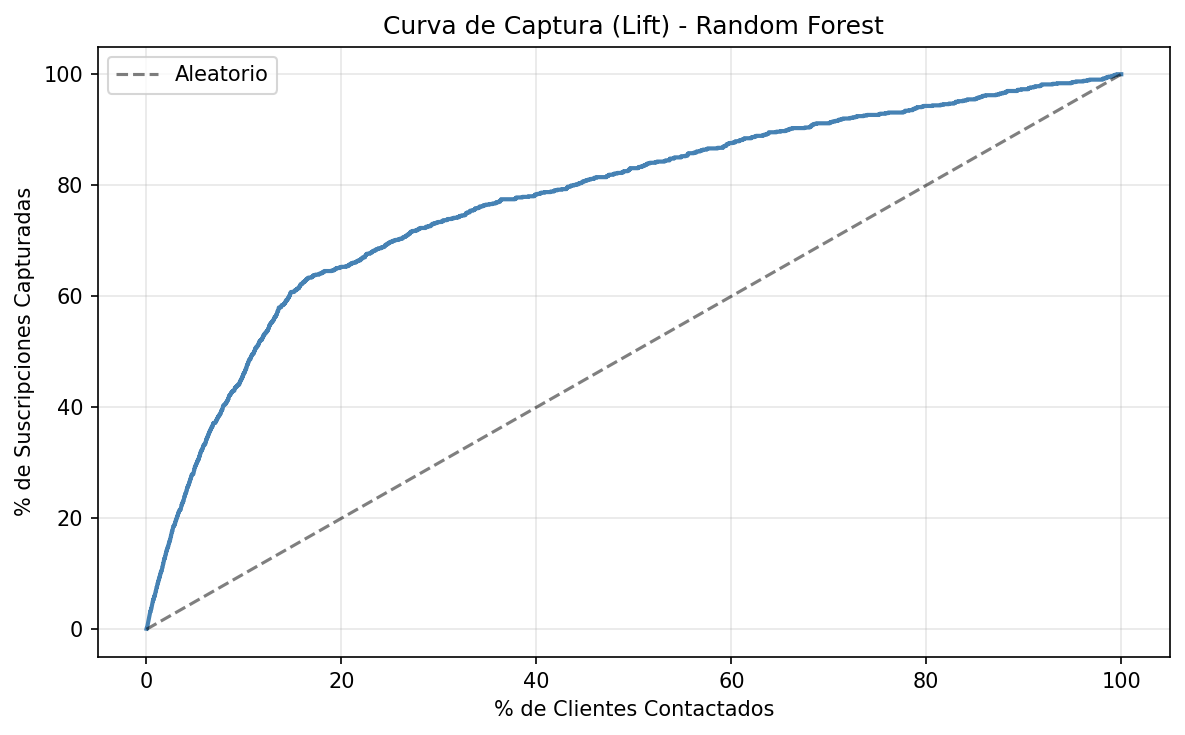
\includegraphics[scale=0.45]{lift_curve_bank.png}
    \caption{Curva de captura (Lift) del modelo seleccionado}
    \label{fig:lift}
\end{figure}

\subsection{Ejemplos de Predicción}

Se presentan 5 predicciones del set de prueba con el modelo seleccionado (Random Forest tuneado), con muestreo estratificado para incluir ejemplos de ambas clases.

\begin{table}[H]
\centering
\caption{Ejemplos de predicción - Bank Marketing (Random Forest)}
\label{tab:pred_bank}
\begin{tabular}{ccccc}
\toprule
\textbf{\#} & \textbf{Real} & \textbf{Predicción} & \textbf{$P(\text{Suscripción})$} & \textbf{Correcto} \\
\midrule
1 & No & No & 0.2039 & Sí \\
2 & No & No & 0.0538 & Sí \\
3 & Sí & No & 0.0615 & No \\
4 & Sí & Sí & 0.5287 & Sí \\
5 & No & No & 0.0445 & Sí \\
\bottomrule
\end{tabular}
\end{table}

El ejemplo \#3 ilustra un falso negativo: un cliente que sí suscribió pero recibió una probabilidad baja (0.0615), probablemente porque su perfil no coincidía con los patrones típicos de conversión. El ejemplo \#4 muestra una predicción correcta de suscripción con $P = 0.5287$, superando el umbral de decisión. Estos ejemplos reflejan las dificultades inherentes del dataset con $\sim$11\% de tasa base positiva.

% ================================================================
% REFERENCIAS
% ================================================================
\begin{thebibliography}{9}

\bibitem{wine}
P. Cortez, A. Cerdeira, F. Almeida, T. Matos, and J. Reis. Wine Quality. \textit{UCI Machine Learning Repository}, 2009. \url{https://doi.org/10.24432/C56S3T}

\bibitem{bank}
S. Moro, P. Cortez, and P. Rita. Bank Marketing. \textit{UCI Machine Learning Repository}, 2014. \url{https://doi.org/10.24432/C5K306}

\bibitem{hastie}
T. Hastie, R. Tibshirani, and J. Friedman. \textit{The Elements of Statistical Learning}, 2nd ed. Springer, 2009.

\bibitem{james}
G. James, D. Witten, T. Hastie, and R. Tibshirani. \textit{An Introduction to Statistical Learning}. Springer, 2013.

\end{thebibliography}

\section{Declaración de Uso de Inteligencia Artificial}

Para la resolución de este examen y la generación del código base en Python, se utilizó el modelo de lenguaje Gemini. A continuación, se detallan los prompts principales utilizados para guiar el análisis:

\begin{itemize}
    \item Prompt utilizado para el Ejercicio 1 (Wine Quality):
\end{itemize}

``Necesito que resuelvas la Practical Question 1 del examen de Statistical Learning (USFQ). El dataset es UCI Wine Quality. Debes: (1) justificar si modelar como regresión, clasificación multiclase o binaria; (2) realizar EDA visual y numérico sobre pH, sulphates, alcohol, volatile acidity y class imbalance; (3) comparar Ridge, Lasso, Elastic Net, Decision Tree, Random Forest, SVM y una red neuronal pequeña; (4) usar k-fold CV para selección de modelo con test set final separado; (5) discutir la estabilidad de predictores Lasso vs Elastic Net; (6) reportar métricas y dar interpretación de negocio para vinicultores.''

\begin{itemize}
    \item Prompt utilizado para el Ejercicio 2 (Bank Marketing):
\end{itemize}

``Necesito que resuelvas la Practical Question 2 del examen de Statistical Learning (USFQ). El dataset es UCI Bank Marketing. Debes: (1) explorar class imbalance, variables categóricas, valores missing-like y variables de campaña; (2) definir un pipeline con imputación, encoding, scaling y chequeo de leakage con duration; (3) comparar modelos lineales regularizados, Decision Tree, Random Forest, SVM y red neuronal; (4) usar stratified CV y reportar ROC-AUC, PR-AUC, recall a precisión fija y confusion matrices a umbrales de negocio; (5) interpretar feature importance sin claims causales; (6) recomendar estrategia de contacto bajo capacidad limitada.''

\end{document}
